\section{Panel fitting}

To obtain the screw adjustments we define an internal region for each panel in the and fit a plane function or a deformed plane function. 
The deformed plane function is shown in equation \ref{eq:deformed_plane} where the deformation is given by the quadratic terms $d$ and $e$. The reduction pipeline gives the option of just use the pure plane function without deformation or the deformed plane function.

\begin{equation}
    z = a+bx+cy+d(x^2+y^2)+e(x^2-y^2)
    \label{eq:deformed_plane}
\end{equation}

To obtain the screw adjustments we evaluate the fitted function in the screw positions to obtain its height, then the adjustment will be the one that brings the screw height to zero. 

Note that this method is valid only when the panel can be correctly represented as a plane, since the changes in the height in the screws positions will generate a tilt or a piston movement, therefore all the other points in the surface will be adjusted correctly.

In the case when the panel is deformed this stops to be true, since now we want to adjust the screws to generate a deformation that reverts the one that the panel already has. So we will need to modify the conversion between height-screw adjustment for the case of deformed panels, this is an on going work.



The figure \ref{fig:plane_panel_fit} shows the overall output of the panel fitting with a plane functions, whereas the figure \ref{fig:deform_panel_fit} shows the output of the panel fitting using the deformed plane function.

The figures \ref{fig:plane_example} and \ref{fig:deform_example} makes a zoom in the panel 411 and shows the debugging tool to examine the panel fitting output. In the case of the panel 411 it can be seen that it has a deformation that connot be well represented by the pure plane function.




\begin{figure}
    \centering
    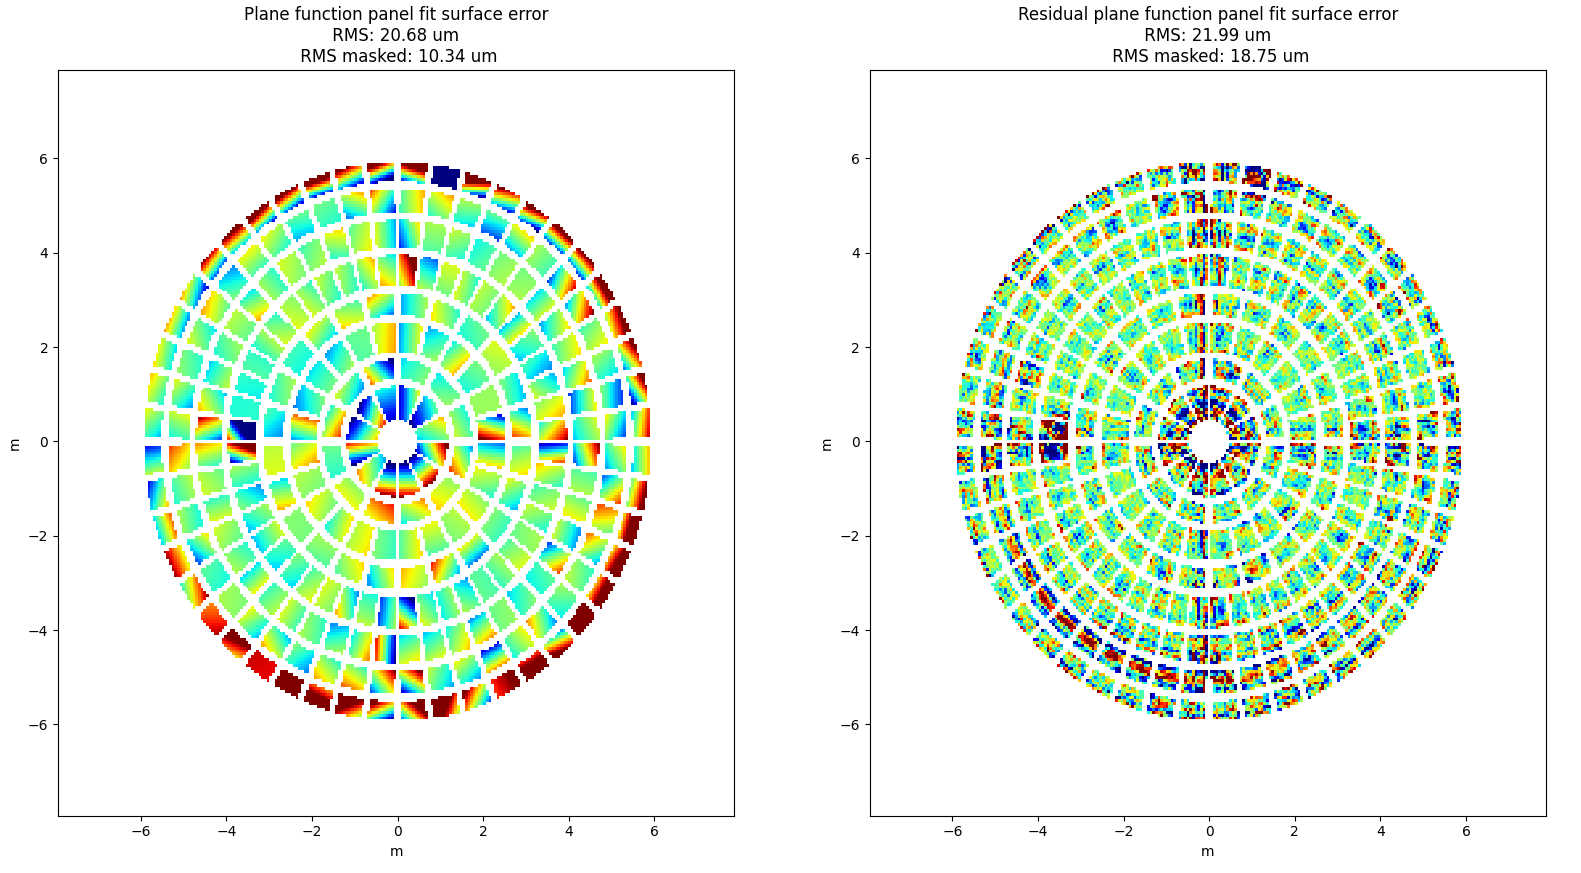
\includegraphics[width=0.8\textwidth]{images/plane_panel_fit.png}
    \caption{Plane panel fitting output.}
    \label{fig:plane_panel_fit}
\end{figure}


\begin{figure}
    \centering
    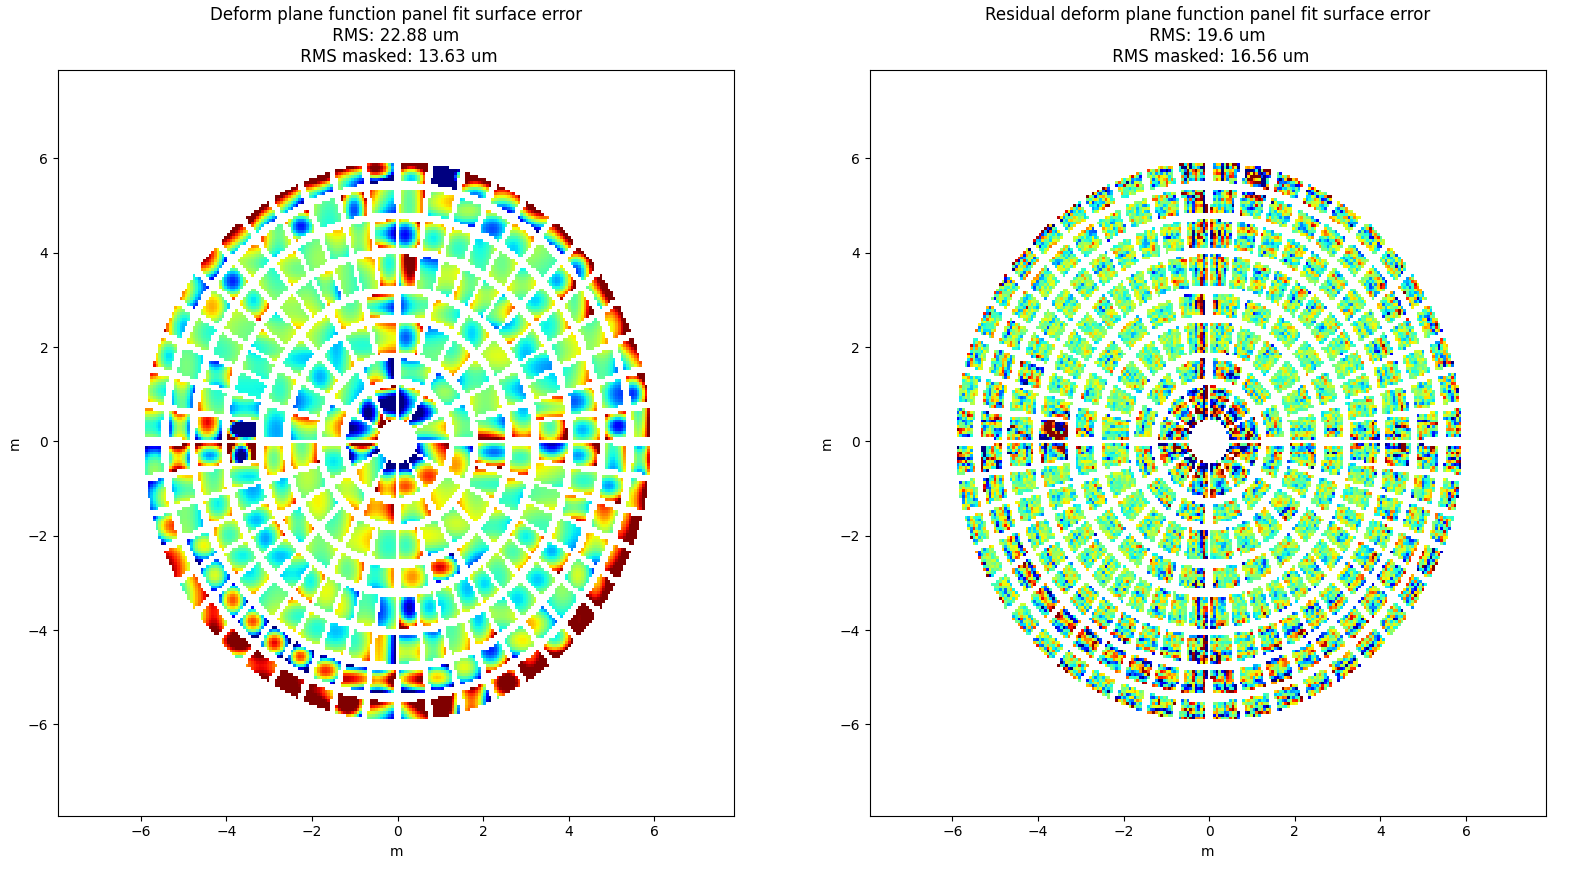
\includegraphics[width=0.8\textwidth]{images/deform_plane_panel_fit.png}
    \caption{Deform plane panel fitting output.}
    \label{fig:deform_panel_fit}
\end{figure}


\begin{figure}
    \centering
    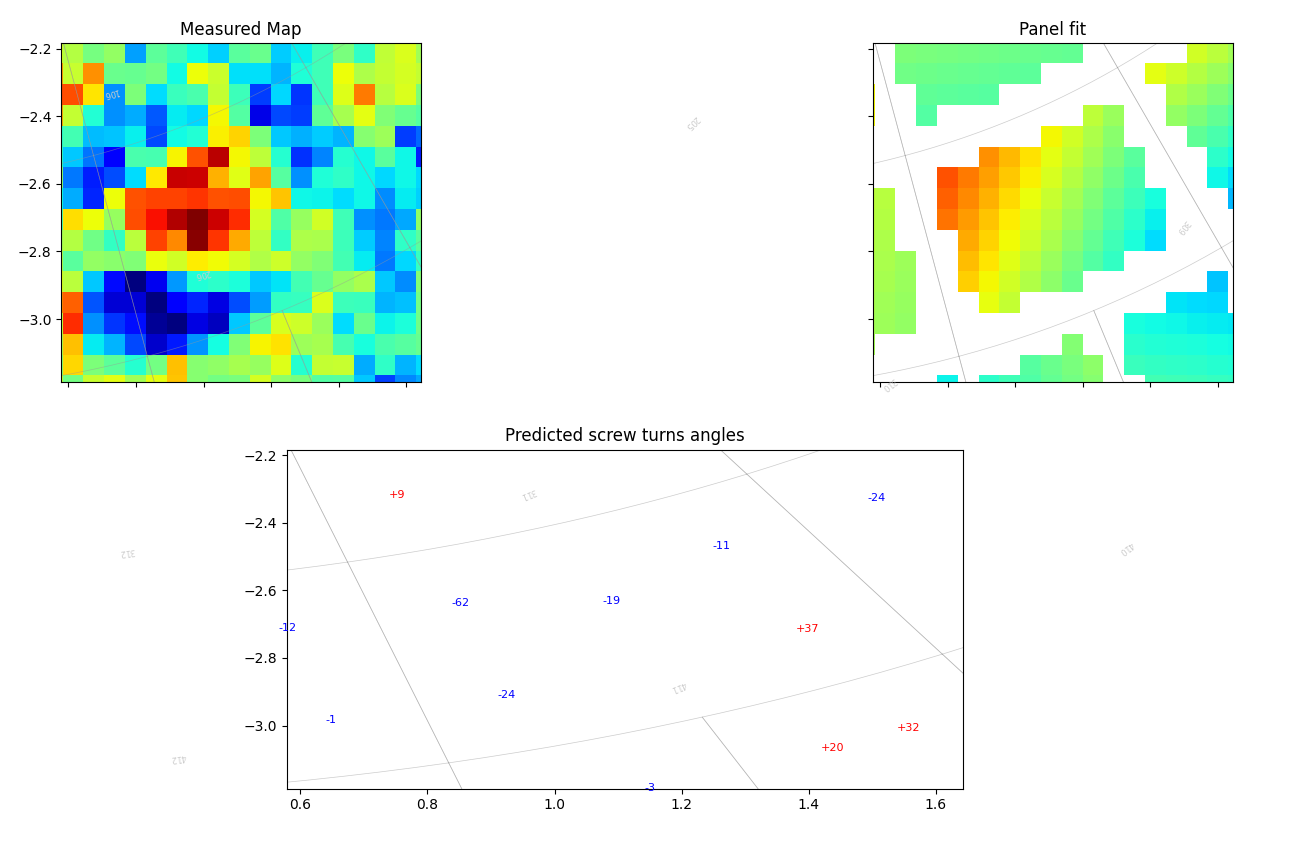
\includegraphics[width=0.8\textwidth]{images/plane_example.png}
    \caption{Debugging tool to view the measured map, the fit surface and the screw adjustments. In this case the fitting procedure was made using a pure plane function and this particular panel is deformed.}
    \label{fig:plane_example}
\end{figure}

\begin{figure}
    \centering
    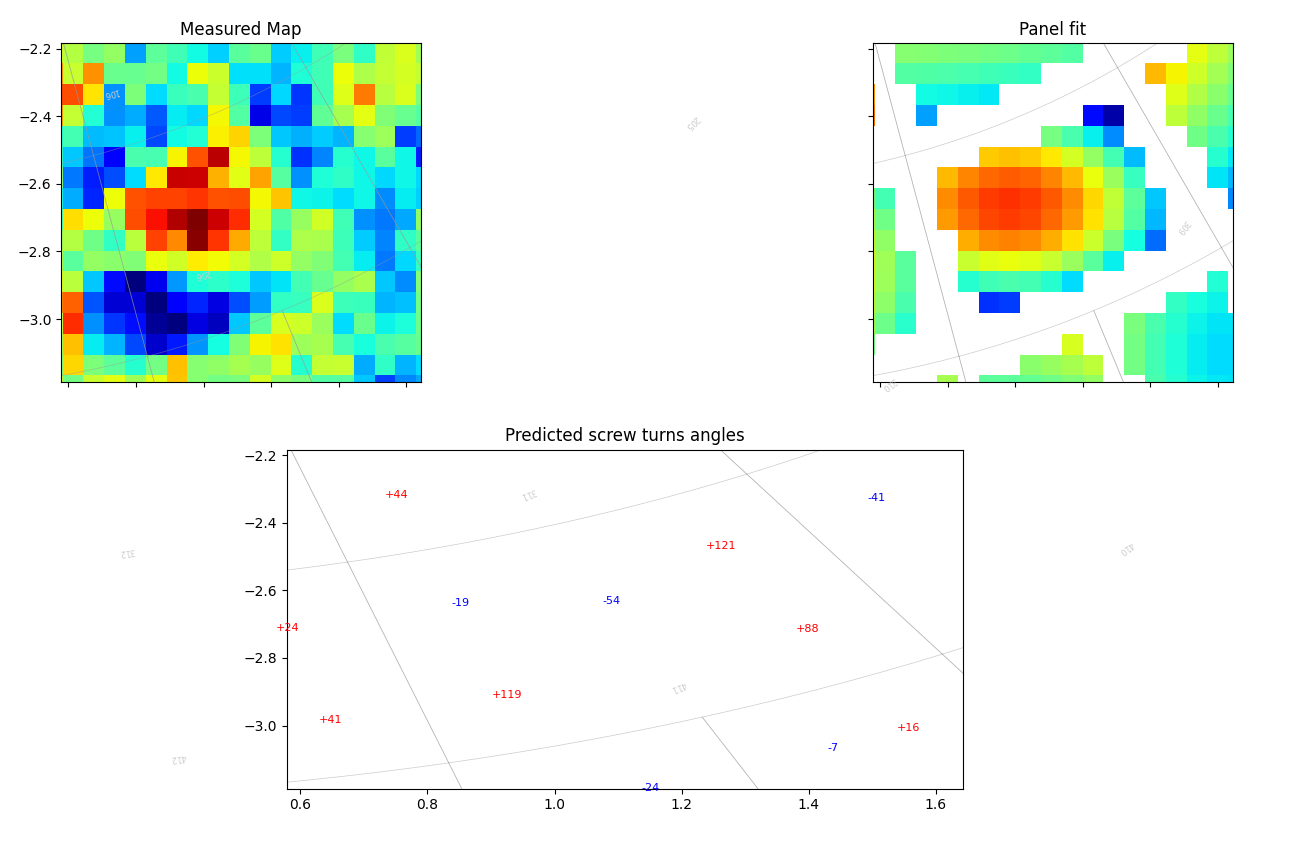
\includegraphics[width=0.8\textwidth]{images/deform_example.png}
    \caption{Debugging tool to view the measured map, the fit surface and the screw adjustments. In this case the fitting procedure was made using a deformed plane function.}
    \label{fig:deform_example}
\end{figure}








